\chapter{Stand van zaken}
\label{ch:stand-van-zaken}

% Tip: Begin elk hoofdstuk met een paragraaf inleiding die beschrijft hoe
% dit hoofdstuk past binnen het geheel van de bachelorproef. Geef in het
% bijzonder aan wat de link is met het vorige en volgende hoofdstuk.

% Pas na deze inleidende paragraaf komt de eerste sectiehoofding.

\section{JavaScript}
\label{sec:JavaScript}

In dit onderdeel zal ten eerste de historiek van JavaScript beschreven worden. Hierna zullen de eigenschappen van JavaScript ten opzichte van andere programmeer talen besproken worden. 

\subsection{Historiek}
\label{sec:JavaScript_Historiek}

JavaScript is uitgevonden in 1995 bij Netscape Communications. Zij hebben ook de Netscape browser gemaakt. In die tijd was Java de populaire taal voor het web. Hierdoor hebben ze besloten om de syntax van JavaScript op die van Java te baseren. De eerste versie van JavaScript was onder de naam Mocha in 1995. Hierna werd deze hernoemd naar LiveScript. Ten slotte werd de taal verandert naar JavaScript eind 1995.
JavaScript is gestandaardiseerd bij ECMA International. Deze gestandaardiseerde versie van JavaScript noemen we ECMAScript. Deze gedraagt zich hetzelfde in alle applicaties die deze standaard accepteren.

\subsection{Eigenschappen}
\label{sec:JavaScript_Eigenschappen}

Het is een object georiënteerde en dynamisch getypeerde scripttaal die gebruikt word om webpagina’s interactief te maken. Deze bevat een standaard bibliotheek van objecten zoals Array, Date en Math. Deze kunnen dan gebruikt worden om de browser en zijn Document Object Model te besturen. Javascript kan HTML elementen plaatsen en/of verwijderen, reageren op events zoals muisclicks, een formulier indienen en navigeren naar een andere pagina.

JavaScript en Java zijn te vergelijken op sommige vlakken maar ook heel verschillend. JavaScript lijkt op Java omdat het dezelfde uitdrukking syntaxis gebruikt. Dit is de wijze waarop een combinatie van waarden, variabelen, operatoren en functies kan worden uitgedrukt. De verschillen worden vervolgens besproken.

Javascript is een dynamisch getypeerde taal. Dit betekend dat het type van een variabele nog niet gekend is bij de compileer tijd. JavaScript ondersteunt een runtime system dat een klein aantal data types ondersteunt. Deze zijn number, boolean en string. Hierdoor kan tijd bespaard worden bij het maken van een project. Elke variabele word gedeclareerd door var, let of const. Een groot nadeel van zo’n dynamisch getypeerde taal is dat je door typfouten bugs kan maken die zeer moeilijk op te sporen zijn. Daartegenover is Java een statisch getypeerde taal. Dit betekend dat bij Java alle types gekend zijn bij compileer tijd. Het voordeel hiervan is dat er een heleboel checks kunnen gedaan worden door de compiler, hierdoor komen veel triviale bugs niet voor.

JavaScript bied meer vrijheid ten opzichte van Java. Je moet niet elke variabele, klasse of methode declareren. Methodes kunnen niet publiek, privaat of beschermd zijn. Er is ook geen nood om interfaces te implementeren. Parameters en functie retourneerwaarden zijn ook niet expliciet getypeerd. Dit kan veel tijd besparen maar ook voor moeilijk te vinden bugs zorgen.

Java is klasse gebaseerd, objecten zijn onderverdeeld in klassen en instanties. Er bestaat en vaste hiërarchie door de klassen heen. Klassen en instanties kunnen niet dynamisch attributen of methoden toegevoegd krijgen. Anderzijds is JavaScript object georiënteerd. Dit betekent dat er geen verschil gemaakt word tussen types van objecten. Overerving kan bereikt worden met behulp van prototypes. Attributen en methoden kunnen dynamisch aan objecten worden toegevoegd \autocite{Introduction_2018}.

\section{Frameworks}
\label{sec:Frameworks}

In dit onderdeel zal ik het uitgebreid hebben over wat een framework is en de componenten waaruit een framework bestaat.

Een software framework is een set methodes en klassen die ontworpen zijn om het werk van een developer te vereenvoudigen. Het is een abstractie van veel kleine componenten die herbruikbaar zijn waardoor veel tijd gespaard kan worden. Een framework legt ook meestal een bepaalde structuur op bij de developer om de code te implementeren. Dit is goed voor consistente code en zorgt voor minder bugs. Er zijn meerdere onderdelen waaruit een framework kan bestaan en deze worden nader besproken \autocite{clifton_what_2003} \autocite{eskelin_software_2001}.

\subparagraph{Wrapper functie}
\label{sec:Frameworks_Wrapper_Functie}
Een wrapper is een methode om één of meerdere functies te versimpelen, consistentie te geven en/of functionaliteit toevoegen. Een wrapper past het bestaande gedrag aan en zal de functionaliteit niet compleet veranderen.

\subparagraph{Architecturen}
\label{sec:Frameworks_Architecturen}
Een architectuur is een stijl dat specifieke ontwerp patronen gebruikt. Een framework heeft een patroon nodig. Meestal ondersteund een framework het gebruik van meerdere ontwerp patronen. Dit patroon zorgt ervoor dat je een herbruikbare structuur maakt in je project. Eenmaal je een patroon gebruikt is het (bijna) onmogelijk om hier van af te stappen of je moet een grote refactor doen van je hele project.

\subparagraph{Methodologie}
\label{sec:Frameworks_Methodologie}
Een methodologie is de manier waarop iets gedaan kan worden. De methodologie is hoe de interactie tussen dingen gebeurt. Hoe objecten met elkaar kunnen communiceren, hoe met persistentie aanneemt of hoe er gereageerd kan worden op user events.

\section{Benchmarking}
\label{sec:Benchmarking}

In dit deel zal de term benchmarking verder uitgelegd worden, wat er onder deze term verstaan word en wat deze proef ermee wil bereiken. Benchmarking heeft verschillende betekenissen volgens het Engelse woordenboek \textcite{_benchmark_????}, enkele zijn hier opgesomd.

“De kwaliteit van iets meten door het te vergelijken met de geaccepteerde standaard.”

“Een standaard om iets te meten of over iets te oordelen van hetzelfde type.”

“Een bepaalde grens van kwaliteit dat kan gebruikt worden als standaard om andere dingen mee te vergelijken.”

Benchmarking is een belangrijk onderdeel van de informatica wereld. Het word overal gebruikt van hardware benchmarks tot database performance benchmarks. Benchmarking tools zijn meestal één of meerdere programma’s die de performance van een applicatie meten onder bepaalde condities. Het doel van zo’n benchmark is om een eerlijke vergelijking te maken tussen verschillende dingen. In deze proef zullen er benchmarks gebruikt worden om de performance van JavaScript frameworks te vergelijken.


\section{MVC}
\label{sec:MVC}

Om de tests in deze proef zo gelijk mogelijk te laten verlopen zal elke applicatie het MVC (Model View Controller) ontwerp patroon zo goed mogelijk proberen hanteren. In dit onderdeel zal ik de basis van het Model-View-Controller patroon beschrijven.

Het Model View Controller patroon is een software architectuur stijl of ontwerp patroon gebruikt voor seperation of concerns. Alle business logica zal zich bevinden in de Controller. Dit is gescheiden van de View. De data die weergegeven wordt bevind zich in een Model. Het patroon beheert de fundamentele werking en data van de applicatie. Het kan reageren voor requests voor informatie, antwoorden met instructies om de state aan te passen en zelfs observers waarschuwen in event-driven systemen. Naast het MVC patroon zijn er meerdere ontwerp patronen ontwikkeld zoals MVVM (model-view-view-model), MVP (model-view-presenter), MVA (model-view-adapter) en nog veel meer. Deze zullen we niet bespreken in deze proef. Het MVC patroon was veel populairder ten opzichte van deze patronen. Verder zullen we de onderdelen van MVC nog kort bespreken \autocite{atwood_understanding_2008} \autocite{_model-view-controller_2014}.

\subparagraph{Model}
\label{sec:MVC_Model}
Ten eerste zal het model besproken worden. Het model definieert de vorm van de data die de applicatie gebruikt. Een model kan een object zijn maar kan ook uit meerdere objecten bestaan. Het model en wat de gebruiker waarneemt hebben meestal een één-op-één relatie. Een model is dus blind, dit betekend dat de model enkel instaat voor de data bij te houden wat er verder met de data gebeurd weet de model niets van. De daadwerkelijke opslag van data wordt door een database gedaan.

\subparagraph{View}
\label{sec:MVC_View}
Informatie wordt weergegeven aan de gebruiker via de view. De view doet geen bewerkingen of berekeningen en dient enkel en alleen om data weer te geven. De user kan op de view bepaalde componenten aanklikken dat events kan triggeren. Deze kunnen doorgezonden worden naar de controller.

\subparagraph{Controller}
\label{sec:MVC_Controller}
De controller kan events opvangen en hierop reageren. Meestal worden er dan bewerkingen uitgevoerd op waarden uit de model. De model word dan aangepast en hierdoor zal de view dan weer geupdate worden.

\section{JavaScript Frameworks}
\label{sec:JavaScript_Frameworks}

In dit hoofdstuk gaan we alle gekozen JavaScript frameworks bespreken samen met hun basisprincipes. Daarna zal bij elk framework in detail besproken worden hoe het renderen gebeurt. Dit heeft namelijk een groot effect op performance.

JavaScript wordt alsmaar populairder met de toename aan frameworks en libraries die gemaakt worden. Voor dit project zijn er drie frameworks gekozen om te vergelijken. De gekozen frameworks zijn React, Angular en Vue. De reden waarom deze gekozen zijn, is omdat deze de drie ‘populairste’ frameworks zijn op dit moment. Hierdoor is er meer ondersteuning en vernieuwing door de community. Ten slotte word er op elk framework iets dieper ingegaan en meerdere basisbegrippen van elk framework worden besproken. Om te bepalen welke frameworks het populairste zijn werd er gekeken naar hoeveel sterren, watchers en forks het framework heeft op GitHub \autocite{github_front-end_????}.

\subsection{Angular}
\label{sec:JavaScript_Frameworks_Angular}
Versie op moment van schrijven: Version 6.0.2

Angular is een framework om applicaties te bouwen met HTML en Typescript. Angular zelf is ook geschreven in Typescript. De basis bouwstenen die Angular op dit moment aanbiedt zijn module, component en service.
Alle informatie over deze basisprincipes komt uit de officiële documentatie van Angular \autocite{_angular_2018}.

\subsubsection{Module}
\label{sec:Angular_Module}
Angular apps zijn modulair. Dit betekent dat de applicatie bestaat uit modules. Zo een module is een bouwsteen code die zich bezighoudt met een bepaald domein van de applicatie, een bepaalde workflow of een gerelateerd stuk code. In een module kan je componenten en services vinden. De scope van deze onderdelen is bepaald door deze module. Een module kan functionaliteit van een andere module importeren maar ook eigen functionaliteit exporteren. De module bepaald zelf welke functionaliteit het open stelt voor andere modules.

\subparagraph{Module metadata}
Een module is een klasse met een @NgModule decorator. Deze decorator neemt 1 metadata object als parameter. Dit object zal de module beschrijven.

De belangrijkste attributen zijn de volgende:
\begin{itemize}
	\item Declarations: Alle components, directives en pipes dat deze module bevat.
	\item Exports: Alles dat andere modules moeten kunnen importeren.
	\item Imports: Andere modules die nodig zijn voor deze module.
	\item Providers: Services worden hier gemaakt, ze worden beschikbaar voor de hele module. Je kan providers ook op component niveau aanmaken. Dit is meestal de voorkeur.
	\item Bootstrap: Dit is het algemene applicatie scherm. De root component. Deze moet in elke module als bootstrap property gezet worden.
\end{itemize}

Modules voorzien een compilatie context voor hun componenten. Tijdens de bootstrap wordt er voor elke module een root component aangemaakt. Hierin komen alle componenten van deze module. Een module kan een willekeurig aantal componenten hebben.

\subsubsection{Component}
\label{sec:Angular_Component}
Een component is een kleine bouwsteen op het scherm, meestal wordt dit een view genoemd. Een bouwsteen kan gaan van kleine dingen zoals knoppen, tot grotere gehelen zoals een form, een kalender of een lijst van items.

De taak van een component is om data weer te geven en acties van de gebruiker door te sturen. Hierdoor blijven componenten puur en eenvoudig. Data ophalen van de server, user input valideren en logica is de taak van services. Services worden later uitgelegd.

Je maakt een component met een klasse, hierin komt alle logica om met de view in te werken. Angular zorgt ervoor dat componenten gecreëerd, bijgewerkt en verwijdert worden. De app die je maakt kan hier gebruik van maken door in te springen op deze lifecycle hooks. Hier word later meer uitleg over gegeven.

\subparagraph{Component metadata}
Een component is een klasse met een @Component decorator. Deze decorator neemt net zoals bij een module 1 metadata object als parameter.

De belangrijkste attributen van dit object zijn:
\begin{itemize}
	\item Selector: Dit is een CSS selector. Een CSS selector zorgt ervoor dat een instantie van deze component in de template HTML word gestopt waar Angular een overeenkomstige tag vind. Als de tag ‘app-button’ is dan zal Angular op alle plekken waar ‘<app-button />’ staat deze component invoegen.
	\item TemplateUrl: Dit is het adres dat de component zal hebben ten opzichte van de module.
	\item Providers: Dit is een Array van services dat de component nodig heeft. Angular zal hierdoor weten welke instanties er nodig zijn om deze component aan te maken.
\end{itemize}

\subparagraph{Component template}
The component template is geschreven in de template syntax. Op het eerste zicht ziet dit er gewoon uit als HTML. Hierbij zit er dan nog de Angular template syntax. Dit bestaat uit data binding, directives en pipes. Met data binding kan je data tonen, met pipes kan je data transformeren voor je ze toont en directives dienen om app logica toe te passen op de data die je toont.

\subsubsection{Service}
\label{sec:Angular_Service}
Een service is een bepaalde functie die een app nodig heeft om te draaien. Deze service heeft meestal 1 bepaald doeleind. Bijvoorbeeld alle functies om 1 bepaald soort objecten uit een database te halen of een form valideren. Op deze manier kan je components klein houden en kan je services hergebruiken.

Componenten gebruiken services, je kan een service injecteren in een component. Zo geef je deze component de mogelijkheid om deze service te gebruiken. Om een service klasse te definiëren maak je een klasse met de @Injectable decorator. Deze zorgt ervoor dat je de service als dependency in een component kan stoppen onder providers.

Angular gebruikt het principe genaamd Dependency Injection. Dit wordt doorheen het hele Angular framework gebruikt om in dit geval services aan components te geven. De injector zorgt hiervoor. Deze moet niet aangemaakt worden, Angular maakt deze aan. Als een component een service nodig heeft gaat de injector kijken of er al een instantie is van deze service. Enkel als deze nog niet aanwezig is zal een nieuwe instantie aangemaakt worden.

\subsubsection{Rendering en Updaten van de view}
\label{sec:Angular_Rendering_Updaten}
Nu alle basisbegrippen van dit framework uitgelegd zijn kunnen we het hebben over het renderen van pagina’s en/of componenten. Dit is een belangrijk onderdeel om de theoretische snelheid te kunnen begrijpen van een framework. Verder in deze proef zal hetzelfde gedaan worden voor elk ander framework. Alle informatie uit dit hoofdstuk is gevonden in de officiële Angular documentatie \autocite{_angular_2018} en artikels van \textcite{precht_thoughtram_2016} en \textcite{koretskyi_angular_2017}.

Op het eerste zicht lijkt het proces zeer simpel. Als een data binding in Angular verandert van waarde dan zal de view hernieuw gerenderd worden. Achter dit simpele principe zit echter een zeer ingewikkeld systeem. Om dit te begrijpen zal ik het eerst hebben over de interne representatie van een applicatie in Angular.

Voor elke component die gebruikt wordt zal een factory method gemaakt worden. Daarna zal Angular de components maken aan de hand van deze factory. Deze factory wordt gebruikt om de view definition op te stellen. De view definition zal hierna gebruikt worden om de component view te maken. Angular representeert de pagina als een boom structuur van views.

De component factory zal een referentie teruggeven naar een viewDef functie. Deze functie maakt de view definition aan. De view definition ontvangt view definition nodes als parameters en deze stellen de structuur van de HTML voor maar kunnen ook Angular details inhouden. De twee belangrijkste nodes die wij gaan bespreken zijn element definition nodes en text definition nodes.

\subparagraph{Element definition}
Een element definition is een node dat Angular genereerd voor elk HTML element en voor componenten. Zo’n element node kan andere element nodes en/of tekst nodes als children hebben. De node heeft een bepaalde paramter genaamd bindings. Dit is de enige waarin wij geïnteresseerd zijn voor de render.

\subparagraph{Text definition}
De text definition node wordt gebruikt door Angular om een text node te maken. Dit is een zeer simpele definitie die beschrijft hoe de tekst eruit zal zien en wordt weergegeven als een array. Deze array zal hierna dan gebruikt worden om de bindings te genereren.

\subparagraph{Update renderer}
De update renderer is een functie dat de factory retourneerd. Deze functie neemt twee parameters de prodCheckAndUpdate functie en de view. De eerste parameter staat voor check en de tweede parameter staat voor de component view met de nodes. De updateRenderer functie wordt opgeroepen als angular veranderingen gaat detecteren bij een component. De parameters zullen worden doorgegeven door het mechanisme dat veranderingen detecteerd.

De taak van de updateRenderer is om de prodCheckAndUpdate functie op te roepen voor elke node en veranderingen te zoeken in de nodes.

\subparagraph{De DOM updaten}
Nu we alle definities kennen die we nodig hebben om te verstaan hoe Angular componenten genereerd kunnen we zien hoe een DOM update gedaan word.

Hierboven is uitgelegd hoe de updateRenderer de functie prodCheckAndUpdate als parameter heeft. Deze functie zal uitgevoerd worden en hieruit zullen meerdere functies vloeien zoals checkAndUpdateElementInline voor element nodes en checkAndUpdateTextInline voor text nodes.

De checkAndUpdateElement functie zal checken of de properties van de node aangepast zijn.

De checkAndUpdateText functie zal checken of de waarden van de tekst aangepast zijn ten opzichte van de vorige check. De vorige waarde zal opgeslagen worden in de oldValues property van de text node.

Indien er veranderingen gebeurd zijn bij deze functies zal Angular de gepaste renderer gebruiken om de DOM te updaten. We zien ook dat elke component voor zichzelf updaten verantwoordelijk is.

\subparagraph{Zones}
Nu we weten hoe componenten geupdate en rerendered worden is er nog één vraag die beantwoord moet worden. Wie zegt nu tegen Angular wanneer er checks gedaan moeten worden en wanneer we deze moeten uitvoeren?

Deze functionaliteit is in Angular geïmplementeerd door middel van zones. Een zone is een object dat een methode run bevat. Met deze run methode kunnen we functies uitvoeren. De functies worden nog steeds uitgevoerd zoals het hoort en hebben hun normaal gedrag. De functionaliteit dat een zone toevoegt zijn bepaalde hooks. Standaard zijn deze hooks onZoneCreated, beforeTask, afterTask en onError. Wat een zone nu zo speciaal maakt zijn precies deze hooks. De volgende functies worden aanzien als een task door een zone: setInterval, alert, prompt, requestAnimationFrame, addEventListener en removeEventListener. Al deze tasks kunnen onderschept worden door de hooks. Angular gaat dus gewaarschuwd worden door zijn zones telkens er een bepaald gedrag uitgevoerd word. Hierdoor zal de view hernieuw gerenderd kunnen worden waardoor het gevolg van dit gedrag zichtbaar wordt.

\subsection{Vue}
\label{sec:JavaScript_Frameworks_Vue}
Versie op moment van schrijven: v2.5.2

Vue is een framework dat geïnspireerd is op het MVVM patroon. Het connecteert de view en de model met behulp van two way data-binding. Een Vue project bestaat over één root Vue instantie. Hierna verdeeld in een boom van herbruikbare components.
Alle informatie over de basisprincipes in Vue komt uit de officiële Vue documentatie \autocite{_vue_2018}.

\subsubsection{Component}
\label{sec:Vue_Component}
In Vue is een component conceptueel hetzelfde als in Angular. Dit concept zullen we zien bij elke framework en is ook de grootste gelijkenis tussen alle frameworks. Vue beschrijft zelf zijn components als een abstractie dat ons de mogelijkheid geeft om grootschalige applicaties te bouwen. Deze kunnen dan bestaan uit kleine zelf onderhouden en meestal herbruikbare components. De meeste interfaces kunnen geabstraheerd worden in een boom van components.

Een component in Vue is in principe een Vue instantie met vooraf gedefinieerde opties. Een component wordt met behulp van onderstaand fragment gemaakt.

\codefragment{code/VueComponent.js}{Vue component voorbeeld}

Deze component kunnen we nu gaan gebruiken in een andere component zijn template. Dit doen we door de component gewoon in de HTML te stoppen. Dit kunnen we vergelijken met de HTML template uit Angular.

\codefragment{code/VueComponentTemplate.html}{Vue component template voorbeeld}

Net zoals bij angular kunnen we met de component template gaan data binden. In vue kunnen we dit met de volgende syntax.

\codefragment{code/vueComponentDatabinding.js}{Vue datat binding in template voorbeeld}

Alles binnen deze haakjes zal als een string worden geïnterpreteerd. Er is maar 1 expressie toegestaan binnen de haakjes. 

\subsubsection{Data}
\label{sec:Vue_Data}
Als er een Vue instantie aangemaakt wordt dan kan je hierin een data object stoppen. Vue zal dit data object blijven bekijken. Als er iets aanpast in dit data object dan zullen de views of components ‘reageren’ en zullen de waarden vernieuwd worden met de nieuwe waarden.

Indien de objecten die je toevoegt aan dit data object niet gedeclareerd zijn vanaf het begin dan zal Vue hier niet op reageren. Je moet alle data een initiële waarde geven.

Objecten kunnen ook niet bekeken of gevolgd worden door Vue als je ze vastzet. Dit kan met de methode ‘Object.freeze()’. Vue zal het nu niet merken als je dit object aanpast.

\subsubsection{Lifecycle Hooks}
\label{sec:Vue_Lifecycle}
Net zoals we gezien hebben in Angular heeft Vue ook Lifecycle methoden. Een paar voorbeelden zijn created, updated en destroyed. Deze kunnen gebruikt worden om data klaar te zetten.

In de Vue documentatie staat er een waarschuwing. Als men gebruik maakt van deze methoden let je best op met de scope van je functies. Indien je lambda functies gebruikt zal de scope wijzen naar de ouder context in plaats van de vue instantie.

\subsubsection{Rendering en Updaten van de view}
\label{sec:Vue_Rendering_Updaten}
Net zoals bij Angular zullen we na deze basisbegrippen uitgelegd te hebben het hebben over het renderen en updaten van de view. Vue gebruikt hiervoor het concept van een Virtual DOM. De Virtual DOM als begrip en idee werd eerst geïntroduceerd door React. Hierna zijn vele andere frameworks dit concept ook gaan gebruiken waaronder ook Vue. Alle informatie in dit hoofdstuk komt uit de officiële Vue documentatie \autocite{_vue_2018-1} en het artikel van \textcite{mikami_medium_2017}.

De Virtual DOM is simpelweg een JavaScript object dat de DOM voorsteld. Het is net zoals de gewone DOM een boomstructuur die alle elementen beschrijft. Je applicatie zal de Virtual DOM updaten en nooit directe manipulaties doen op de DOM.

Zoals geweten is manipulaties doen op de DOM een dure bewerking. De echte DOM wordt meteen gerenderd in de browser als je hem update. Met behulp van een Virtual DOM kunnen we meerdere bewerkingen op de dom bijhouden en nadien tegelijk uitvoeren op de echte DOM. Het tweede voordeel dat zo’n Virtual DOM biedt is dat je kan kiezen welk deel opnieuw gerenderd moet worden. Stel dat je pagina 10 elementen telt maar er wordt er maar één aangepast. Hiervoor heeft de Virtual DOM een functie die kan vinden welk element er is aangepast en deze enkel gaan aanpassen in de DOM.

Vue zal bij het builden van de applicatie je templates omzetten naar een Virtual DOM. De values van data bindings zullen in de Virtual DOM de waarde krijgen die ze op dat moment hebben. Het voordeel om de templates om te zetten bij build time is dat er performance kan gespaard worden door dit niet in de runtime te doen.

\subparagraph{Het proces}
Nu we in grote lijnen weten hoe Vue zijn componenten zal renderen kunnen we het hebben over het proces. In dit deel zullen we het beknopt hebben over hoe Vue dit proces uitvoert.

Het eerste wat hiervoor besproken zal worden is de defineProperty functie deze functie zal opgeroepen worden telkens je het Data object van een component aanpast. De defineProperty functie zorgt ervoor dat elk data object een getter en setter krijgt.

Als we zo’n set function oproepen en het Data object dus gaan updaten zal Vue de Watcher gaan aanspreken. Dit zijn objecten binnen de Vue Virtual DOM. Een Watcher zal aangemaakt worden voor elke component als de applicatie geïnitializeerdt word. De taak van deze watcher zal zijn om de Virtual DOM en de DOM te updaten. Maar zal dit niet meteen doen.

Het moment dat de Watcher aangesproken word zal hij zichzelf toevoegen aan een wachtlijst. Hierdoor wordt vermeden dat de Watcher meerdere maal uitgevoerd zal worden. De Watcher wordt namelijk elke keer er een setter aangeroepen word uitgevoerd. Als een Data object nu 10 variabelen heeft zal deze 10 keer aangeroepen worden vlak na elkaar. Nadat de Watcher in de wachtlijst komt zal de wachtlijst opgeruimd worden en gesorteerd worden. Het opruimen gebeurt door dubbele Watchers samen te voegen.

De laatste stap van dit proces is de nextTick API. Deze Vue functie zal alle Watchers uitvoeren en doorspoelen in de wachtlijst. Eenmaal alle Watchers uitgevoerd en doorgespoeld zijn zal de DOM geupdate worden. Na al deze stappen zal de DOM geupdate worden in de Watcher zijn run functie. De run functie kan ook handmatig aangeroepen worden om een force rerender aan te roepen. De Watchers die elk verantwoordelijk zijn voor hun eigen component zullen hier dus elk hun eigen component gaan updaten in de Virtual DOM en de DOM.

In het volgende en laatste hoofdstuk zullen we bespreken hoe het laatste framework React het re-renderen en updaten van de view afhandelt.


\subsection{React}
\label{sec:JavaScript_Frameworks_React}
Versie op moment van schrijven: v16.3.2

Volgens React is het een declaratieve, effectieve en flexibele JavaScript library om interfaces te bouwen. Het is inderdaad een libary, maar de mogelijkheden die React biedt leiden tot veel discussie of het nu een library of een framework is. In dit onderzoek werd React ook gekozen omdat het samen met de twee andere frameworks bij de drie populairste methodes hoort voor web development. De reden dat tot deze discussie leidt is omdat React enkel de view voorziet. React bestaat uit een virtuele DOM die gebruikt wordt voor het efficiënt re-renderen van de DOM. Hiernaast zijn er ook components die een eigen state hebben.
Alle informatie over de basisprincipes in React komt uit de officiële React documentatie \autocite{_react_2018}.

\subsubsection{Component}
\label{sec:React_Component}
In React is het mogelijk op een component op verschillende manieren te declareren. De belangrijkste manier is de React.Component klasse. In dit geval is de component een klasse die React.Component zal overerven.

\codefragment{code/ReactComponent.js}{React component voorbeeld}

Een component als deze heeft minstens één methode namelijk ‘render()’. Deze methode geeft een descriptie van wat je wilt renderen. Dit noemen we een React element. Een React element is een uitleg van wat je wil weergeven op het scherm. De syntax van de ‘render()’ methode lijkt enorm op HTML maar is eigenlijk een syntax genaamd JSX. React zorgt ervoor dat de component correct kan weergegeven worden in de browser wanneer er data aangepast wordt.

De tweede methode om componenten te maken noemen we functional components. Deze syntax is korter wat wilt zeggen ook eenvoudiger. In plaats van een klasse te declareren die ‘React.Component’ extend kunnen we ook een functie schrijven die teruggeeft wat we willen renderen.

\codefragment{code/ReactFunctionalComponent.js}{React functional component voorbeeld}

Nu de twee methoden uitgelegd zijn om een component aan te maken wordt er meer uitleg gegeven over wat een component inhoud. Elke component heeft een ‘props’ parameter. Via de props kan data doorgegeven worden aan child components. Props worden doorgegeven in de JSX syntax in de render.

\codefragment{code/ReactChildComponent.js}{React parent met child component voorbeeld}

Elke React component heeft ook een state. Als de state van een component aanpast zal React de components proberen re-renderen. React zal dit enkel en alleen doen indien dit nodig is voor de gebruiker.

\subsubsection{Rendering en Updaten van de view}
\label{sec:React_Rendering_Updaten}
In dit onderdeel zal ik voor React uitleggen hoe het renderen en updaten van een view in zijn werk gaat. Net zoals bij Vue zal React werken met een Virtual DOM. React is namelijk het eerste framework dat met deze render oplossing is gekomen. Zij hebben dit concept ook verder uitgewerkt. Alle informatie uit dit hoofdstuk komt uit de officiële React documentatie \autocite{_react_2018} en de artikels van \textcite{mishra_hackernoon_2017} en \textcite{kurian_medium_2017}.

Als in React de state aagepast word dan zal een component gemarkeerd worden als ‘dirty’. Alle DOM event listeners zijn in React omhult in hun eigen event listeners. Hierdoor wordt door elke muisklik of ander event een naamloze functie van React opgeroepen worden. Als een component zijn state aangepast wordt dan zal die gemarkeerd worden als ‘dirty’.

Nu is de component gemarkeerd als dirty. Ten eerste zullen we de component updaten als batch update. Dit betekend dat als de state meerdere keren vlak na elkaar aangepast word React maar 1 keer zal rerenderen. Hierna zal er nogmaals gekeken worden of de state aangepast is of er een forceUpdate aangeroepen werd.

Hierna zullen we de hele lifecycle doorlopen van de React component. In dit onderdeel gaan we dieper ingaan op één bepaalde lifecycle methode namelijk render. React zal nu de Virtual DOM aanpassen. Het concept van een Virtual dom werd reeds uitgelegd bij Vue.

Het moment waarop de Virtual DOM heropgebouwd word zal React kijken of het vorige en volgende element van hetzelfde type en sleutel zijn. Indien dit niet het geval is zal het dit overeenstemmen. Hierna zal de DOM geupdate worden met de components die in de Virtual DOM aangepast zijn in één keer.

\subsection{Data binding}
\label{sec:Data_Binding}
Elk framework gebruikt het concept data bindings. Er bestaan 2 types data binding. One-way data binding en two-way data binding.

Traditionele server-side web applicaties maken gebruik van one-way data binding. Hier word een template en data modellen samengevoegd en verzonden naar de gebruiker zijn browser. Alle aanpassingen die gemaakt worden moeten dus via de server gebeuren en er zal een nieuwe view verstuurd moeten worden naar de browser. One-way data binding is voorgesteld met behulp van een schema in figuur \ref{fig:one_way_data_binding}

\begin{figure}[h!]
	\caption{One-way data binding \autocite{_data_????}}
	\centering
	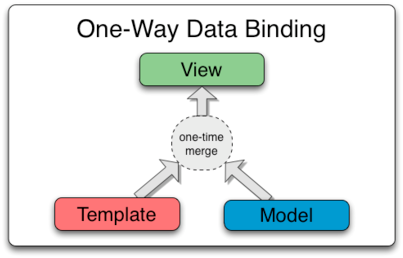
\includegraphics[width=7cm]{img/onewaydatabinding.png}
	\label{fig:one_way_data_binding}
\end{figure}

De meest gebruikte methode van data binding in JavaScript Frameworks is two-way data binding. De view is hierbij een directe projectie van het model. Dit betekend dat alle aanpassingen door de gebruiker meteen aangepast worden in het model en omgekeerd worden ook alle aanpassingen in het model meteen zichtbaar in de view. Two-way data binding is voorgesteld met behulp van een schema in figuur \ref{fig:two_way_data_binding}

\begin{figure}[h!]
	\caption{Two-way data binding \autocite{_data_????}}
	\centering
	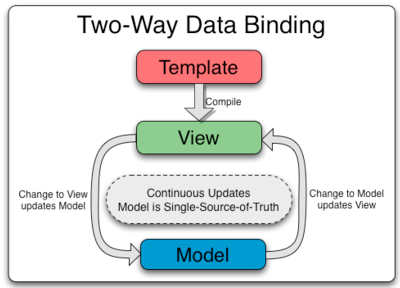
\includegraphics[width=7cm]{img/twowaydatabinding.png}
	\label{fig:two_way_data_binding}
\end{figure}

\subsection{Application state}
\label{sec:Application_state}
De state van een applicatie is de plek waar data vandaan komt. Om een webapplicatie interactiever te maken zijn er meer states nodig. Bij server side rendering of one-way data binding is het moeilijker om kleine aanpassingen te maken. Dit is bij webapplicaties die gebouwd zijn met JavaScript frameworks makkelijker te implementeren. Hierdoor hebben zo’n webapplicaties meestal een complexere state. De state van een applicatie kan op verschillende manieren aangepast worden:

\begin{itemize}
	\item I/O in forms, fields kunnen gevalideerd worden.
	\item Interactie met knoppen kan een nieuwe pagina tonen.
	\item Data van de API kan aankomen.
\end{itemize}

\section{Vergelijking criteria}
\label{sec:Vergelijking_Criteria}

\subsection{Theoretische vergelijking}
\label{sec:Theoretische_Vergelijking}
In dit onderdeel zullen we alle criteria bespreken die we kunnen afleiden uit het literatuur onderzoek en de bronnen. Eerst worden alle criteria opgesomd.

\subparagraph{Populariteit}
Een populair framework gebruiken is voordelig in vele aspecten. Het is ook zeer belangrijk voor de stabiliteit van het framework. Een developer vind veel informatie op StackOverflow en andere fora. Hier worden problemen besproken en opgelost door mede-developers. Een grote developer gebruikers aantal kan ervoor zorgen dat bugs sneller gerapporteerd worden. Daarnaast zullen deze bugs ook sneller kunnen opgelost worden. Naast deze voordelen zorgt de grote populariteit er ook voor dat er veel libraries gemaakt en ondersteund worden voor dit framework.

\begin{itemize}
	\item Wat zijn de resultaten op Google Trends van deze drie frameworks? Google Trends geeft een goede indicatie over hoe populair een framework is en hoe veel developers ernaar zoeken. Het geeft ook een indicatie naar hoe de populariteit stijgt of daalt.
	\item Wat zijn de resultaten op StackOverflow Trends van deze drie frameworks? StackOverflow Trends geeft een goede indicatie over hoeveel informatie je kan vinden over deze frameworks. Een probleem oplossen is altijd apart maar sommige gelijkaardige problemen kunnen al opgelost zijn op StackOverflow. Hierdoor kan tijd bespaard worden.
	\item Hoeveel GitHub watchers telt het framework? Hoe meer mensen het project volgen op github hoe meer development versies getest kunnen worden. Hierdoor kunnen features sneller gepubliceerd worden.
\end{itemize}

\subparagraph{Security}
Tegenwoordig slaat bijna elke site gevoelige of persoonlijke info op in een database die verbonden staat met het internet. Door de groei van het web word dit als maar meer en meer data. De veiligheid van deze data is zeer belangrijk. Een security breach kan mogelijk de informatie lekken van vele gebruikers en het vertrouwen kan hierdoor verloren worden. Hiervoor gaan we een paar criteria opnemen in deze proef.

\begin{itemize}
	\item Voorkomt het framework Cross Site Request Forgery? Cross site request forgery is een veiligheidsprobleem waarbij de gebruiker gedwongen wordt om acties uit te voeren die hij niet wil. Deze aanval gaat niet om data diefstal. Het is een aanval waarbij de aanvaller de state van de applicatie manipuleert.
	\item Voorkomt het framework Cross Site Scripting? Cross site scripting zijn een soort van injectie waardoor kwaadaardige scripts geïnjecteerd worden in vertrouwbare websites. De gebruiker’s browser heeft geen manier om te valideren of de scripts te vertrouwen zijn.
\end{itemize}

\subparagraph{Bruikbaarheid}
De bruikbaarheid en developer vriendelijkheid van een framework zijn belangrijk. Door bepaalde repetitieve code te genereren kan er veel tijd bespaard worden. Sommige talen zoals TypeScript zorgen er voor dat er minder fouten op typering kunnen gemaakt worden. Deze factoren kunnen de bruikbaarheid van het framework verbeteren.

\begin{itemize}
	\item Bestaat er een tool om code te genereren? In plaats van herhaalbare code te blijven schrijven bespaard code generatie veel tijd voor een developer.
\end{itemize}

\subparagraph{Stabiliteit}
Er is geen enkele methode die ons toestaat om de stabiliteit van een framework te meten. We kunnen dit proberen achterhalen door te kijken hoe wijd gebruikt het framework is.

\begin{itemize}
	\item Wordt het framework gebruikt door een grote organisatie? Als een groot bedrijf dit framework gebruikt kan het een indicatie zijn naar hoe stabiel het framework is. Dit is ook een indicatie naar hoe dit bedrijf staat ten opzichte van deze technologie in de toekomst.
\end{itemize}

\subparagraph{Compatibiliteit}
JavaScript wordt uitgevoerd in de browser en het is belangrijk dat het framework ondersteund word door zo veel mogelijk browsers. Mobiele apparaten zijn ook een belangrijk onderdeel, een groot deel van de gebruikers gebruikt zijn mobiel toestel om te surfen op het internet.

\begin{itemize}
	\item Ondersteunt het framework mobiele apparaten? Tegenwoordig bestaat het grootste deel van de internet gebruikers uit mobiele apparaten. Het is dus belangrijk om deze te ondersteunen.
\end{itemize}

\subparagraph{Modulair}
Het doel van modulair zijn is om structuur te geven aan de developer. Een voorbeeld van modulair zijn is het gebruik van componenten. Een component is namelijk een geïsoleerde eenheid die vervangen kan worden. Het maakt het makkelijker om de gehele applicatie te onderhouden.

\begin{itemize}
	\item Heeft de framework een specifiek ontwerp patroon waardoor het development van verschillende lagen of componenten makkelijker word? Zoals hierboven vermeld is het belangrijk om structuur en vervangbaarheid te hebben in een project. 
	\item Ondersteund het framework een component gebaseerde methodologie? Werken met componenten is cruciaal geworden in het hedendaagse web development. Componenten kunnen makkelijk vervangen of verplaatst worden zonder de gehele applicatie te beïnvloeden.
\end{itemize}

\subparagraph{Testing}
Het is belangrijk dat de frameworks getest kunnen worden. Veel development teams gebruikten een test-driven development methode. Dit zorgt ervoor dat aanpassingen de applicatie niet stuk maken en dat nieuwe functionaliteit getest kan worden voor release. Testen zijn belangrijk omdat software bugs zeer duur of zelfs gevaarlijk kunnen zijn voor de gebruiker.

\begin{itemize}
	\item Ondersteund het framework unit tests? Unit tests zorgen ervoor dat de functionaliteit van bepaalde modules correct werkt.
	\item Ondersteund het framework integratie tests? Integratie tests zorgen ervoor dat de gehele applicatie getest kan worden.
\end{itemize}

\subsection{Praktische vergelijking}
\label{sec:Praktische_Vergelijking}
In dit onderdeel zullen alle metrieken besproken worden die getest worden in deze proef. Er worden twee soorten metrieken besproken. De eerste soort zullen meten op software complexiteit en de tweede soort op performance.

\subparagraph{First meaningfull paint}
First meaningfull paint is de tijd waarop de applicatie initieel laad en is cruciaal bij de gebruiker. De eerste momenten waarop een webstie laad geven de gebruiker een gevoel hoe performant de website is. Hoe kleiner deze initiële tijd is hoe beter.

\subparagraph{Grootte}
De grootte van de applicatie is te zien in de Chrome netwerk tab. Hoe kleiner deze file hoe minder de gebruiker zal moeten downloaden. Dit zorgt ook voor een sneller en performanter gevoel. Deze pijler hangt af van te grootte van het framework en extra afhankelijkheden die we toevoegen in het project. Om dit zo eerlijk mogelijk te laten verlopen zal in elk project zo min mogelijk afhankelijkheden toegevoegd worden. Zo kan elk framework zo correct mogelijk vergeleken worden.

\subparagraph{Tarief}
Het tarief is het aantal werk dat een framework kan doen binnen een bepaalde tijdspanne is een belangrijke factor bij performance. Dit is ook cruciaal voor de gebruiker. Het tarief zullen we meten aan de hand van meerdere tests. Elke test zal een verschillende hoeveelheid werk hebben. We gaan testen hoe lang het duurt voor een framework om een variabel aantal entiteiten te veranderen.








